\documentclass{article}
\usepackage{graphicx}
\usepackage[utf8]{inputenc}
\usepackage[T1]{fontenc}
\usepackage{imakeidx}
\usepackage{hyperref}
\usepackage{listings}
\usepackage{amsthm}
\usepackage{float}

\makeindex
\hypersetup{
colorlinks,
linkcolor=blue,
urlcolor=blue,}


\title{Git for Robots}   
\author{Arjun Gandhi} 
\date{\today} 

\begin{document}

%theroms definitions
\newtheorem*{definition}{Definition}
\newtheorem*{concept}{Concept}
\newtheorem{golden-rule}{Golden Rule}

%=========================================
\begin{titlepage}
		\centering{
			{\fontsize{40}{48}\selectfont 
			Git for Robotics}
		}\\
			
		\vspace{10mm}
		\centering{\Large{Arjun Gandhi}}\\
		\vspace{\fill}
		\centering \large{March 2020}
\end{titlepage}


%=========================================
\newpage{}
\thispagestyle {empty}

\vspace*{2cm}

\begin{figure}
    \centering
	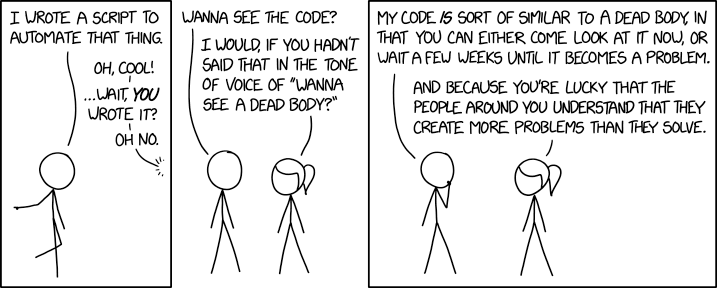
\includegraphics[width=5.5in]{images/wanna_see_the_code.png}
	\caption{This is how all of my robotics project go.}
\end{figure}

\newpage
{
\hypersetup{
linkcolor=black,
urlcolor=black,}

\tableofcontents

}

\newpage
\section{What is version control?}

    You can think of a version control system (short: "VCS\index{version control system}") as a kind of "database". It lets you save a snapshot of your complete project at any time you want. When you later take a look at an older snapshot (let's start calling it "version\index{version}"), your VCS shows you exactly how it differed from the previous one.
    \begin{figure}[hp]
    \centering
    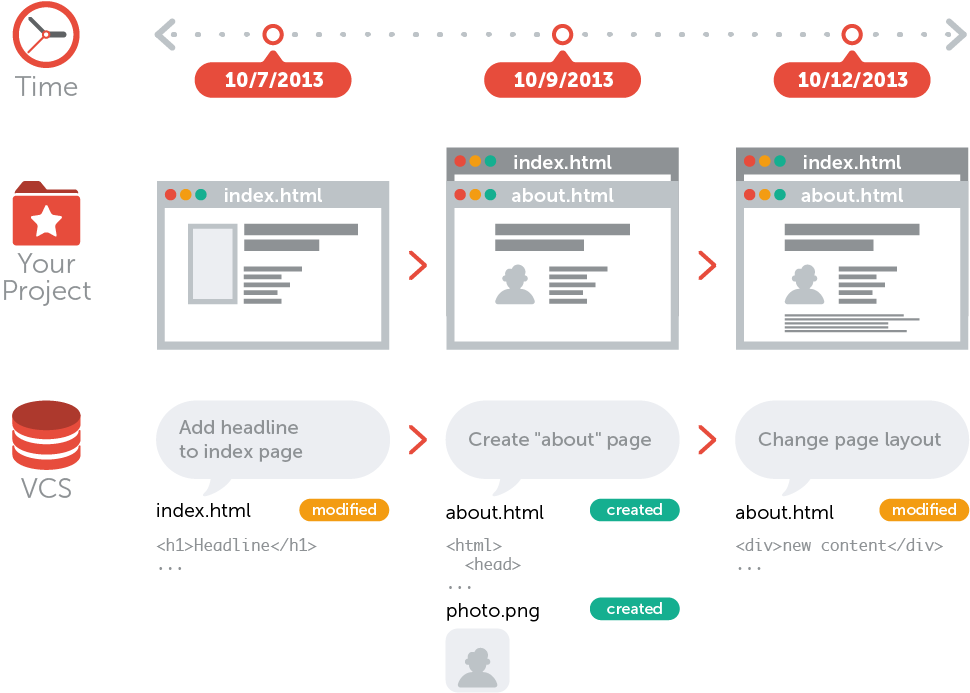
\includegraphics[width=4.5in]{images/what_is_vcs.png}
    \end{figure}
    \newline
    Version control is independent of the kind of project / technology / framework you're working with:
    \begin{itemize}
        \item It works a website as it does for a robotics project
        \item It lets you work with any tool you like; it doesn't care what kind of text editor, graphics program, file manager or other tool you use
    \end{itemize}
    At the core of it a VCS records the changes you make to your project's files. This is what version control is about. It's really as simple as it sounds.
\subsection{Why use version control}
    
    With out a VCS you are probably working together in a shared folder on the same set of files. Texting your teammates that you are currently working on file "xyz" and that, meanwhile, your teammates should keep their fingers off. This is an awful idea. It's extremely error-prone as you're essentially doing open-heart surgery all the time: sooner or later, someone will overwrite someone else's changes.
    \newline\newline
    With a VCS, everybody on the team is able to work absolutely freely - on any file at any time. The VCS will later allow you to merge all the changes into a common version. There's no question where the latest version of a file or the whole project is. It's in a common, central place: your version control system.
    \newline\newline
    Other benefits of using a VCS are even independent of working in a team or on your own.
    
    \subsubsection{Storing Versions (Properly)}
    Making a save of your project after you make critical changes is an important and necessary habit. It prevents you from losing your new work and allows you to go back to your old work easily in case you need it. Without a VCS your save system might look like the following awful ideas (I have personally seen someone do every one of these).
    \begin{itemize}
        \item Saving the changes as a new file and appending a number/date to the end.
        \item Making a copy of the entire code and pasting it (commented out) below the actual code for each version of the code. 
        \item Copying the code and sending it in an email.
        \item Saving pictures of the code and putting them in Dropbox.
        %add more fun bad examples if you can think of it
    \end{itemize}
    The core of this however is that the problem gets out of hand fast. 
    \newline\newline
    A VCS solves this problem. A version control system acknowledges that there is only one project. Therefore, there's only the one version on your disk that you're currently working on. Everything else - all the past versions and variants - are neatly packed up inside the VCS. When you need it, you can request any version at any time and you'll have a snapshot of the complete project right at hand.
    \subsubsection{Restoring Old Versions}
    Being able to restore older versions of a file (or even the whole project) effectively means one thing: you can't mess up! If the changes you've made lately prove to be garbage, you can simply undo them in a few clicks. Knowing this should make you a lot more relaxed when working on important bits of a project.
    
    \subsubsection{Understanding What Changes Were Made}
    When working in large teams understanding what changes other members have done quickly is crucial to efficient working. 
    \newline\newline
    Every time you save a new version of your project, your VCS requires you to provide a short description of what was changed. Additionally (if it's a code / text file), you can see what exactly was changed in the file's content. This helps you understand how your project evolved between versions.
    
    \subsubsection{Backup}
    It's happened to all of us before you accidental deleted a critical file in a moment of panic. Luckily a side-effect of using a distributed VCS like Git is that it can act as a backup; every team member has a full-blown version of the project on his disk - including the project's complete history. Should your beloved central server break down (and your backup drives fail), all you need for recovery is one of your teammates' local Git repository.
    
    \subsubsection{What is Git?}
    By far, the most widely used modern version control system in the world today is Git. Git is a mature, actively maintained open source project originally developed in 2005 by Linus Torvalds, the famous creator of the Linux operating system kernel. A staggering number of software projects rely on Git for version control, including commercial projects as well as open source. Developers who have worked with Git are well represented in the pool of available software development talent and it works well on a wide range of operating systems and IDEs (Integrated Development Environments).
    
\section{Setting Up}
There are two main ways of working with Git: either via its "Command Line Interface" or with a GUI application. Neither of these are right or wrong.
\newline\newline
On the one hand, using a GUI application is likely easier at first and can help new users with the basic features.
\newline\newline
On the other hand, however, I recommend learning the basics of Git on the command line first. It helps you form a deeper understanding of the underlying concepts and makes you independent from any specific GUI application.
\newline\newline
In this guide we will be using to command line interface not only because of the foundations it provides but also as it is what you will be using in the later robotics classes.
\newline\newline
There are also several well designed third party applications, I recommend checking them out after you get a handle on git.*
\newline\newline
*Note: Downloading a third party app is may not be supported by the RBE Department, this is due to the authentication process 


\subsection{Setting Up Git on Your Computer}
Installing Git has become incredibly easy in recent times. There are one-click installers for both Mac and Windows.
\newline\newline
In this tutorial, like in many others, the "\$" sign represents the prompt of the command line interface (you don't have to type this character in your commands!). Therefore, any time you see a line starting with the "\$" sign, it means we're executing commands in "Terminal" or "Git Bash".


\subsubsection{Installing Git on Windows}
On Windows, you can download the "Git for Windows" package from here: \href{https://git-for-windows.github.io/}{ https://git-for-windows.github.io/}  
Allow popup: yes
\newline\newline
When running the installer EXE, you should choose the default options in each screen. After finishing the installation, you can begin working with Git by starting the "Git Bash" application. You'll find it in the Windows START menu, inside the "Git" folder:
\begin{figure}[h]
    \centering
    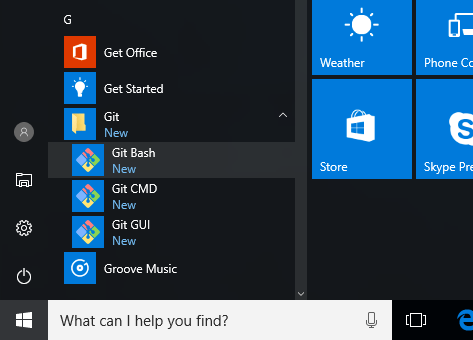
\includegraphics[width=4.5in]{images/git-bash-windows}
\end{figure}

\subsubsection{Installing Git on MacOS}

Download and run the installer from \href{https://sourceforge.net/projects/git-osx-installer/files/}{here}.
Follow the prompts to install Git.
\newline\newline
Note: if you are already using Homebrew, feel free to use that instead with the following command:
\begin{lstlisting}[language=bash]
$ brew install git
\end{lstlisting}
Then open up the terminal you can do this by starting "Terminal.app" on your Mac. You'll find this in the "Utilities" subfolder of your "Applications" folder in Finder:

\begin{figure}[h]
    \centering
    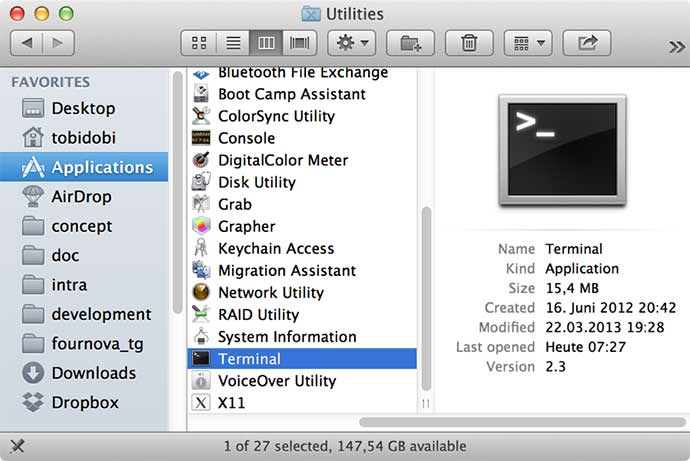
\includegraphics[width=4.5in]{images/terminal-app-mac.jpg}
\end{figure}



\subsubsection{Installing Git on Linux}
Use your the appropriate package manager for your linux system to install git:
\newline\newline
Some of the common systems are listed below.
\newline\newline
Open terminal and run the following commands:
\newline
\textbf{Ubuntu/Debian}

\begin{lstlisting}[language=bash]
$ sudo apt update
$ sudo apt install git
\end{lstlisting}

\textbf{Redhat Based System}
\begin{lstlisting}[language=bash]
$ sudo yum install git
\end{lstlisting}

\textbf{Arch Linux}
\begin{lstlisting}[language=bash]
$ sudo pacman -S git
\end{lstlisting}

\subsection{Setting up GitHub}

To proceed with this process you need to make a GitHub account. 
\newline\newline
If you don't already have one you can sign up for it \href{https://github.com/join?source=header-home}{here}:
\newline\newline
I recommend signing up for a \href{https://education.github.com/pack}{Student Developer Pack}(you get lots of free stuff)
\newline\newline
You do need to send in a picture of your id because of WPI email addresses being weird.

\subsubsection{Configuring Git}
A couple of very basic configurations should be made before you get started. You should set your name and email address as well as enable coloring to pretty up command outputs:
\newline\newline
Make sure to use the same email that you used for your GitHub account.

\begin{lstlisting}[language=bash]
$ git config --global user.name "John Doe"
$ git config --global user.email "john@doe.org"
$ git config --global color.ui auto
\end{lstlisting}

\section{Basic Workflow}

Before we get lost in Git commands, you should understand what a basic workflow with version control looks like. We'll walk through each step in detail later in this book. But first, let's get an understanding of what the workflow in general is like.
\newline\newline
The most basic building block of version control is a "\index{repository}repository".

\begin{definition}Repository:
\newline\newline
Think of a repository as a kind of database where your VCS stores all the versions and metadata that accumulate in the course of your project. In Git, the repository is just a simple hidden folder named ".git" in the root directory of your project. Knowing that this folder exists is more than enough. You don't have to (and, moreover, should not) touch anything inside this magical folder.
\end{definition}

Getting such a repository on your local machine can be done in two ways:

\begin{itemize}
    \item If you have a project locally on your computer that is not yet under version control, you can initialize a new repository for this project.
    \item  If you're getting on board of a project that's already running, chances are there is a repository on a remote server (on the internet or on your local network). You'll then probably be provided with a URL to this repository that you will then "clone" (download / copy) to your local computer.
\end{itemize}


(1)As soon as you have a local repository, you can start working on your files: modify, delete, add, copy, rename, or move files in whatever application (your favorite editor, a file browser, ...) you prefer. In this step, you don't have to watch out for anything. Just make any changes necessary to move your project forward.
\newline\newline
(2)It's only when you feel you've reached a noteworthy state that you have to consider version control again. Then it's time to wrap up your changes in a \index{commit}commit.
\begin{definition}Commit:
\newline\newline
A commit is a wrapper for a specific set of changes. The author of a commit has to comment what he did in a short "commit message". This helps other people (and himself) to understand later what his intention was when making these changes.
\newline\newline
Every set of changes implicitly creates a new, different version of your project. Therefore, every commit also marks a specific version. It's a snapshot of your complete project at that certain point in time (but saved in a much more efficient way than simply duplicating the whole project...). The commit knows exactly how all of your files and directories looked and can therefore be used, e.g., to restore the project to that certain state.
\end{definition}
(3) However, before you commit, you'll want to get an overview of what you've changed so far. In Git, you'll use the "status" command to get a list of all the changes you performed since the last commit: which files did you change? Did you create any new ones or deleted some old ones?
\newline\newline
(4) Next, you tell Git which of your local changes you want to wrap up in the next commit. Only because a file was changed doesn't mean it will be part of the next commit! Instead, you have to explicitly decide which changes you want to include. To do this, you add them to the so-called "Staging Area".
\newline\newline
(5) Now, having added some changes to the Staging Area, it's time to actually commit these changes. You'll have to add a short and meaningful message that describes what you actually did. The commit will then be recorded in your local Git repository, marking a new version of your project.
\newline\newline
(6) From time to time, you'll want to have a look at what happened in the project - especially if you're working together with other people. The "log" command lists all the commits that were saved in chronological order. This allows you to see which changes were made in detail and helps you comprehend how the project evolved.
\newline\newline
(7) Also when collaborating with others, you'll both want to share (some of) your changes with them and receive the changes they made. A remote repository on a server is used to make this exchange possible.

\begin{definition}

 Local \& Remote Repositories\newline\newline
 There are two kinds of repositories:
\newline
A "local" repository resides on your local computer, as a ".git" folder inside your project's root folder. You are the only person that can work with this repository, by committing changes to it.
A "remote" repository, in contrast, is typically located on a remote server on the internet or in your local network. No actual working files are associated with a remote repository: it has no working directory but it exclusively consists of the ".git" repository folder. Teams are using remote repositories to share \& exchange data: they serve as a common base where everybody can publish their own changes and receive changes from their teammates.
\end{definition}

\subsection{Creating a local git repository}
\subsection{Starting with an Unversioned Project}

Let's start with an existing project that is not yet under version control. Change into the project's root folder on the command line and use the "git init" command to start versioning this project:

\begin{lstlisting}[language=bash]
$ cd path/to/project/folder
$ git init
\end{lstlisting}

Now take a moment to look at the files in that directory (including any hidden files):

\begin{lstlisting}[language=bash]
$ ls -la
\end{lstlisting}

You'll see that a new, hidden folder was added, named ".git". All that happened is that Git created an empty local repository for us. Please mind the word "empty": Git did not add the current content of your working copy as something like an "initial version". The repository contains not a single version of your project, yet.

 \newtheorem*{working-copy}{Working Copy}
 \begin{working-copy}
The root folder of your project is often called the "working copy" (or "working directory"). It's the directory on your local computer that contains your project's files.
\newline\newline
You can always ask the version control system to populate your working copy with any version of your project. But you always only have one working copy with one specific version on your disk - not multiple in parallel.
\end{working-copy}

\subsubsection{Ignoring Files}
Typically, in every project and on every platform, there are a couple of files that you don't want to be version controlled: Eclipse likes to make a massive .eclipse folder and if version controlled it has a tendancy to cause problems. In other projects, you might have build or cache files that make no sense in a version control system. You'll have to decide yourself which files you don't want to include.

 \newtheorem*{note}{Note}
 \begin{note}
What Files Should I Ignore?
\newline\newline
As a simple rule of thumb you'll most likely want to ignore files that were created automatically (as a "by-product"): temporary files, logs, cache files...
\newline\newline
Other examples for excluded files range from compiled sources to files that contain passwords or personal configurations.
\newline\newline
A helpful compilation of ignore rules for different projects and platforms can be found \href{https://www.github.com/github/gitignore}{here} 
 \end{note}

The list of files to ignore is kept in a simple file called ".gitignore" in the root folder of your project. It's highly recommended to define this list at the very beginning of your project - before making your first commit. Because once files are committed, you'll have to jump through some hoops to get them out of version control, again.
\newline\newline
Now, let's get going: Create an empty file in your favorite editor and save it as ".gitignore" in your project's root folder. If you're on a Mac, e.g., you'll want to make sure it contains at least the following line:
\newline
\begin{lstlisting}[language=bash]
.DS_Store
\end{lstlisting}

If there are other files you want to ignore, simply add a line for each one. Defining these rules can get quite complex. Therefore, to keep things simple, I'll list the most useful patterns which you can easily adapt to your own needs:
\begin{itemize}
    \item Ignore one specific file: Provide the full path to the file, seen from the root folder of your project.
    \newline
path/to/file.ext
    \item Ignore all files with a certain name (anywhere in the project): Just write down the file's name, without giving a path.
    \newline
filename.ext
    \item Ignore all files of a certain type (anywhere in the project): 
    \newline
    *.ext
    \item  Ignore all files in a certain folder:
    \newline
path/to/folder/*
\end{itemize}

\subsubsection{Making Your First Commit}
With some ignore rules in place, it's time to make our initial commit for this project. We'll go into great detail about the whole process of committing a little later in this book. For now, simply execute the following commands:

\begin{lstlisting}[language=bash]
$ git add -A
$ git commit -m "Initial commit"
\end{lstlisting}

\section{Starting with an Existing Project on a Server}

\subsubsection{Creating a repository on GitHub}
We are going to go onto GitHub and make our first repository.
Log on to Github and hit the new repository button:
\begin{figure}[h]
    \centering
    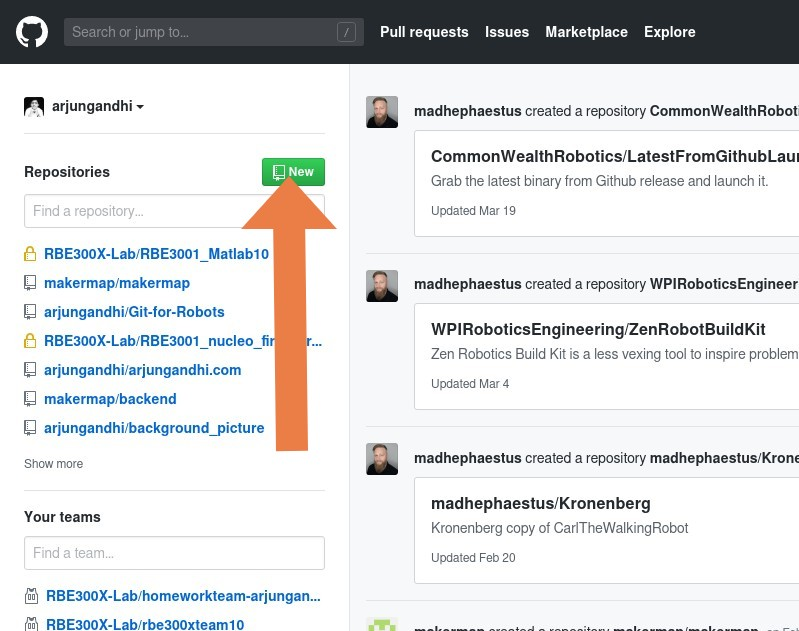
\includegraphics[width=4.5in]{images/new-repo.jpg}
\end{figure}
\newline\newline
Go ahead and give your repository any name you want: 
\begin{figure}[h]
    \centering
    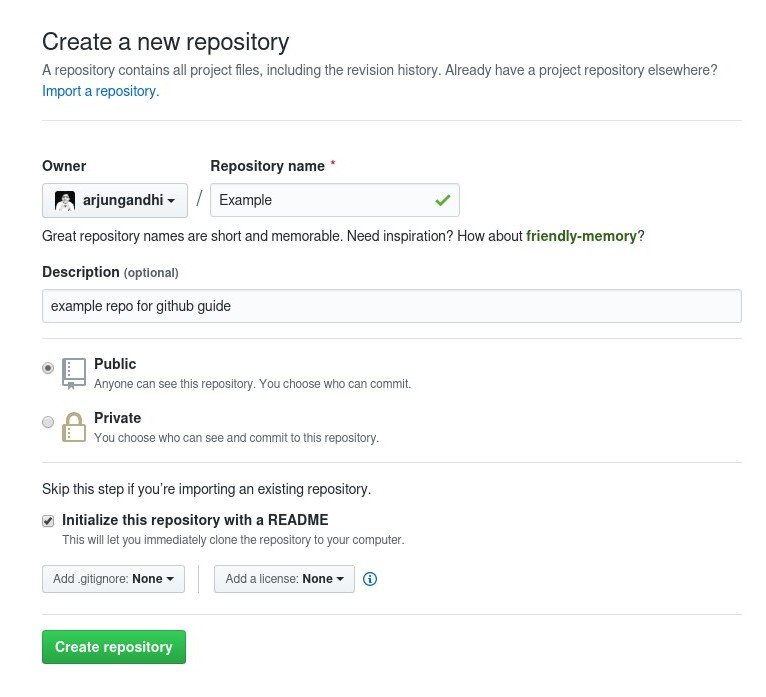
\includegraphics[width=4.5in]{images/new-repo2.jpg}
\end{figure}
\newline\newline
There are a couple options on Github
\begin{itemize}
    \item Public vs Private: This means exactly what you thing choose public if you want to keep the repository to found by others on the GitHub website and private if you want only you and select friends/teamates to be able to see and access the repository
    \item Initialize repository with a Read Me: This will create an example file called README.md in all GitHub repository's this file will be rendered when ever some one visits the repository. This is a good place to put any useful information about the project your working on that some one new might need to know.
\end{itemize}
\newpage
Now we need to download the new GitHub project onto our computer. This is known as \index{clone}cloning a repository.
\newline
\newline
We first need the url for the repository this can be found by clicking the clone or download button on the page.
\begin{figure}[H]
    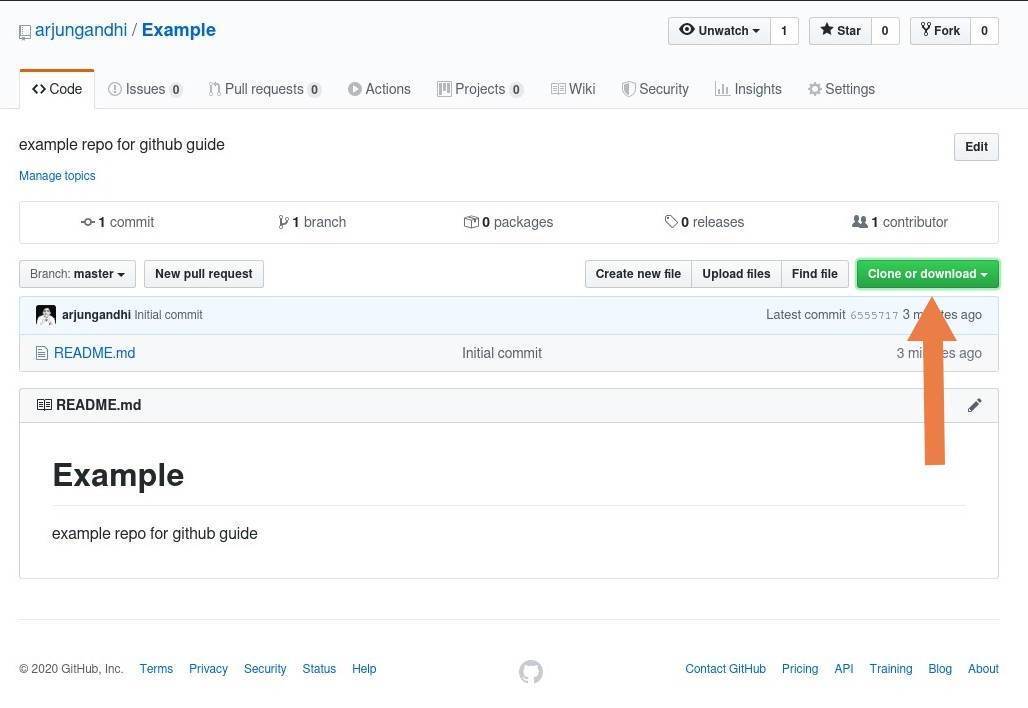
\includegraphics[width=4in]{images/clone.jpg}
\end{figure}
Copy the link that pops up and make sure you have selected the HTTPS option.
\newline\newline
Go back to the terminal and cd into the directory where you want to download the repository.
\begin{lstlisting}[language=bash]
$ cd your/development/folder/
\end{lstlisting}
Now we will clone our new repository with the clone command.
\begin{lstlisting}[language=bash]
$ git clone https://github.com/arjungandhi/Example.git
\end{lstlisting}
You will have to enter your username and password here in this case you will be using your github username and password.

Git will now download a complete copy of this repository to your local disk.

\section{Working on your Project}
No matter if you created a brand new repository or if you cloned an existing one - you now have a local Git repository on your computer. This means you're ready to start working on your project: use whatever application you want to change, create, delete, move, copy, or rename your files.


 \begin{concept}
The Status of a File: 
\newline\newline
In general, files can have one of two statuses in Git:
\begin{itemize}
    \item untracked: a file that is not under version control, yet, is called "untracked". This means that the version control system doesn't watch for (or "track") changes to this file. In most cases, these are either files that are newly created or files that are ignored and which you don't want to include in version control at all.
    \item tracked: all files that are already under version control are called "tracked". Git watches these files for changes and allows you to commit or discard them.
\end{itemize}
 \end{concept}
\subsection{The Staging Area}
At some point after working on your files for a while, you'll want to save a new version of your project. Or in other words: you'll want to commit some of the changes you made to your tracked files.

 \begin{golden-rule}Commit Only Related Changes:
 \newline\newline
When crafting a commit, it's very important to only include changes that belong together. You should never mix up changes from multiple, different topics in a single commit. For example, imagine wrapping both some work for your path planning and your drive code in fix \#169 the same commit:
\begin{itemize}
    \item Understanding what all those changes really mean and do gets hard for your teammates (and, after some time, also for yourself). Someone who's trying to understand the progress of that new login functionality will have to untangle it from the bugfix code first.
    \item Undoing one of the topics gets impossible. Maybe your login functionality introduced a new bug. You can't undo just this one without undoing your work for fix \#169, also!
\end{itemize}
Instead, a commit should only wrap related changes: fixing two different bugs should produce (at the very least) two separate commits; or, when developing a larger feature, every small aspect of it might be worth its own commit.
Small commits that only contain one topic make it easier for other members of your team to understand the changes - and to possibly undo them if something went wrong.
 \end{golden-rule}
However, when you're working full-steam on your project, you can't always guarantee that you only make changes for one and only one topic. Often, you work on multiple aspects in parallel.
 \newline\newline
This is where the "Staging Area", one of Git's greatest features, comes in very handy: it allows you to determine which of your local changes shall be committed. Because in Git, simply making some changes doesn't mean they're automatically committed. Instead, every commit is "hand-crafted": each change that you want to include in the next commit has to be marked explicitly ("added to the Staging Area" or, simply put, "staged").
\begin{figure}[h]
    \centering
    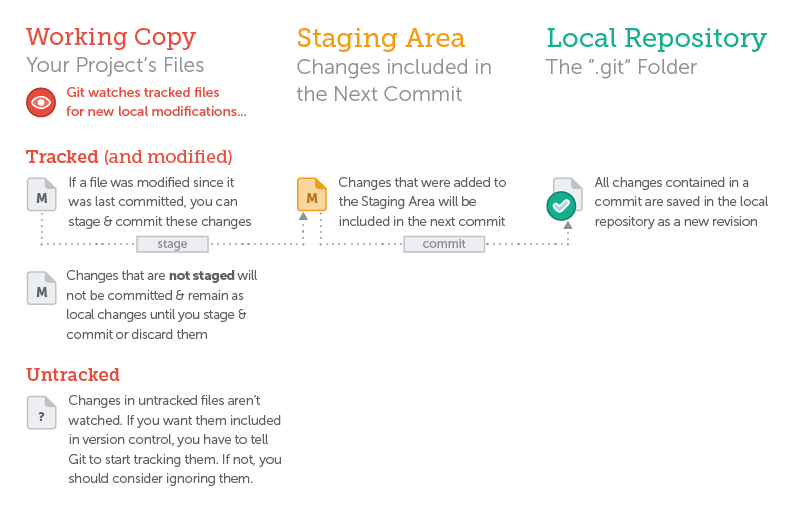
\includegraphics[width=4.5in]{images/staging-area-file-status.png}
\end{figure}


\subsection{Getting an Overview of Your Changes}
Let's have a look at what we've done so far. To get an overview of what you've changed since your last commit, you simply use the "git status" command:
\begin{lstlisting}[language=bash]
$ git status
# On branch master
# Changes not staged for commit:
#   (use "git add/rm <file>... " to update what will be committed)
#   (use "git checkout -- <file>..." to discard changes in working
#    directory)
#
#       modified:   robot/drive.py
#       modified:   robot/path.py
#       deleted:    work.py
#       modified:   runofftable.py
#       modified:   dobackflip.py
#
# Untracked files:
#    (use "git add <file>..." to include in what will be committed)
#       display.py
no changes added to commit (use "git add" and/or "git commit -a")
\end{lstlisting}
Thankfully, Git provides a rather verbose summary and groups your changes in 3 main categories:
\begin{itemize}
    \item "Changes not staged for commit"
    \item "Changes to be committed"
    \item "Untracked files"
\end{itemize}
\subsection{Getting Ready to Commit}
Now it's time to craft a commit by staging some changes with the "git add" command:
\begin{lstlisting}[language=bash]
$ git runofftable.py display.py robot/*
\end{lstlisting}
With this command, we added the new "display.py" file, the modifications in "runofftable.py", and all the changes in the "robot" folder to the Staging Area. Since we also want to record the removal of "work.py" in the next commit, we have to use the "git rm" command to confirm this:
\begin{lstlisting}[language=bash]
$ git rm work.py
\end{lstlisting}
Let's use "git status" once more to make sure we've prepared the right stuff:
\begin{lstlisting}[language=bash]
$ git status
# On branch master
# Changes to be committed:
#   (use "git reset HEAD <file>..." to unstage)
#
#       modified:   robot/drive.py
#       modified:   robot/path.py
#       deleted:    work.py
#       modified:   runofftable.py
#       new file:   display.py
#
# Changes not staged for commit:
#   (use "git add <file>..." to update what will be committed)
#   (use "git checkout -- <file>..." to discard changes in working 
#    directory)
#
#       modified:   dobackflip.py
#
\end{lstlisting}

Assuming that the changes in "dobackflup.py" concerned a different topic than the rest, we've deliberately left them unstaged. That way, they won't be included in our next commit and simply remain as local changes. We can then continue to work on them and maybe commit them later.
\subsection{Committing Your Work}
Having carefully prepared the Staging Area, there's only one thing left before we can actually commit: we need a good commit message.
\begin{golden-rule}Write Good Commit Messages
\newline\newline
Time spent on crafting a good commit message is time spent well: it will make it easier to understand what happened for your teammates (and after some time also for yourself).
\newline\newline
Begin your message with a short summary of your changes (up to 50 characters as a guideline). Separate it from the following body by including a blank line. The body of your message should provide detailed answers to the following questions: What was the motivation for the change? How does it differ from the previous version?
\end{golden-rule}

The "git commit" command wraps up your changes:
\begin{lstlisting}[language=bash]
$ git commit -m "Got the robot to drive off a table consistently"
\end{lstlisting}

If you have a longer commit message, possibly with multiple paragraphs, you can leave out the "-m" parameter and Git will open an editor application for you (which you can also configure via the "core.editor" property).

\begin{concept}What Makes a Good Commit?
\newline\newline
The better and more carefully you craft your commits, the more useful will version control be for you. Here are some guidelines about what makes a good commit:
\begin{itemize}
    \item Related Changes: As stated before, a commit should only contain changes from a single topic. Don't mix up contents from different topics in the same commit. This will make it harder to understand what happened.
    \item Completed Work: Never commit something that is half-done. If you need to save your current work temporarily in something like a clipboard, you can use Git's "Stash" feature (which will be discussed later in the book). But don't eternalize it in a commit.
    \item Tested Work: Related to the point above, you shouldn't commit code that you think is working. Test it well - and before you commit it to the repository.
    \item Short \& Descriptive Messages: A good commit also needs a good message. See the paragraph above on how to "Write Good Commit Messages" for more about this.
\end{itemize}
Finally, you should make it a habit to commit often. This will automatically help you to keep your commits small and only include related changes.

 \end{concept}

If you are working in a repository the commits you made locally arent pushed to the cloud yet. You can do this with the git push command.

\begin{lstlisting}[language=bash]
$ git push
\end{lstlisting}

\subsection{Inspecting the Commit History}
Git saves every commit that is ever made in the course of your project. Especially when collaborating with others, it's important to see recent commits to understand what happened.
\newline\newline
The "git log" command is used to display the project's commit history:
\begin{lstlisting}[language=bash]
$ git log
\end{lstlisting}
It lists the commits in chronological order, beginning with the newest item. If there are more items than it can display on one page, the command line indicates this by showing a colon (":") at the end of the page. You can then go to the next page with the SPACE key and quit with the "q" key.
\begin{lstlisting}[language=bash]
commit 2dfe283e6c81ca48d6edc1574b1f2d4d84ae7fa1
Author: Arjun Gandhi <beepboop@arjungandhi.com>
Date: Fri Jul 26 10:52:04 2013 +0200

    Got the robot to drive off a table consistently

commit 2b504bee4083a20e0ef1e037eea0bd913a4d56b6
Author: Arjun Gandhi <beepboop@arjungandhi.com>
Date: Fri Jul 26 10:05:48 2013 +0200

    Got the robot to unplug its own wires

commit 0023cdddf42d916bd7e3d0a279c1f36bfc8a051b
Author: Arjun Gandgi <beepboop@arjungandhi.com>
Date: Fri Jul 26 10:04:16 2013 +0200

    Robot learned about fire! oh no!
\end{lstlisting}

Every commit item consists (amongst other things) of the following metadata:
\begin{itemize}
    \item Commit Hash
    \item Author Name \& Email
    \item Date
    \item Commit Message
\end{itemize}
 \begin{definition}The Commit Hash:
 \newline\newline
Every commit has a unique identifier: a 40-character checksum called the "commit hash". While in centralized version control systems like Subversion or CVS, an ascending revision number is used for this, this is simply not possible anymore in a distributed VCS like Git: The reason herefore is that, in Git, multiple people can work in parallel, committing their work offline, without being connected to a shared repository. In this scenario, you can't say anymore whose commit is \#5 and whose is \#6.
 \newline\newline
Since in most projects, the first 7 characters of the hash are enough for it to be unique, referring to a commit using a shortened version is very common.
 \end{definition}

Apart from this metadata, Git also allows you to display the detailed changes that happened in each commit. Use the "-p" flag with the "git log" command to add this kind of information:

\begin{lstlisting}[language=bash]
$ git log -p
commit 2dfe283e6c81ca48d6edc1574b1f2d4d84ae7fa1
Author: Arjun Gandhi <beepboop@arjungandhi.com>
Date: Fri Jul 26 10:52:04 2013 +0200

    Got the robot to drive off a table consistently

diff --git a/robot/drive.py b/robot/path.css
index e69de29..4b5800f 100644
--- a/css/drive.py
+++ b/css/drive.py
@@ -0,0 +1,2 @@
+ for pid in pids:
+     pid.dopid()
\ No newline at end of file
diff --git a/robot/path.py b/robot/path.py
index a3b8935..d472b7f 100644
--- a/robot/path.py
+++ b/robot/path.py
@@ -21,7 +21,8 @@
 +edges=lidar.find_edge
+ target=None
+ for edge in edges:
+     if edge.distance > 1000:
+         target = edge.center()
+         break
+ path=astar(cur_pos,target)
+ return path
diff --git a/work.py b/work.py
deleted file mode 100644
index 78alc33..0000000
--- a/work.py
+++ /dev/null
@@ -1,43 +0,0 @@
- robot.begood()
- robot.disable_murphy()
- robot.disable_stupid()
\end{lstlisting}

This shows in detail how each file in the commit was modified or changed. %potentiall add a section on how to interpret this in detal?

\subsection{Time to Celebrate}
Congratulations this is the fundamentals of working with git and version control many projects can and have been build on this foundation. However git can do much more than this. So take a break maybe grab a beverage and lets continue on!
\newline \newline
I suggest to further cementing your knowledge try doing all the actions work on a small programming project. A fun one is to try writing an auto solver for the \href{https://www.24game.com/t-about-howtoplay.aspx}{24 Game}. Remember to keep all the things you have learned in mind about committing often and frequently with good commit messages!

\section{Branching can Change Your Life}
It sounds insane .... But the truth is: it's not an exaggeration. Using branches in your day-to-day work might very well prove to make you a better programmer or designer.
\newline\newline
Now, let's look at why branches are so important.
\subsection{Working in Contexts}
In every project, there are always multiple different contexts where work happens. Each feature, bugfix, experiment, or alternative of your product is actually a context of its own: it can be seen as its own "topic", clearly separated from other topics.
\newline\newline
This leaves you with an unlimited amount of different contexts. Most likely, you'll have at least one context for your "main" or "production" state, and another context for each feature, bugfix, experiment, etc.
\newline\newline
In real-world projects, work always happens in multiple of these contexts in parallel:
\begin{itemize}
    \item While you're experimenting with two verisions of a PID loop to see which one runs faster (context 1 \& 2)...
    \item you're also trying to fix an annoying bug (context 3).
    \item On the side, you also update some set values for your gripper (context 4), while...
    \item one of your teammates is working on brand new gripper code (context 5),...
    \item and another teammate is trying to rewrite the entire codebase (context 6).
\end{itemize}

\subsection{A World Without Branches}

Not working in clearly separated contexts can (and sooner or later will) cause several problems:
\begin{itemize}
    \item What happens if your your 2nd PID codes turns out to be much faster but in the meantime a bunch of other changes have happened
    \item What happens if the new gripper code your teammate wrote turned out to be hot garbage? How do you get all that unwanted code (and only that code!) out?
    \item What do you do if the entire code rewrite turns proves to be impossible to implement? It's already mingled with all of those other changes, being almost impossible to separate out!
    \item How can you avoid losing track? Most likely, you shouldn't be bothered with all the topics from all of your teamates.
\end{itemize}
Things will start to get very confusing when you try to handle multiple topics in a single context:
\begin{figure}[h]
    \centering
    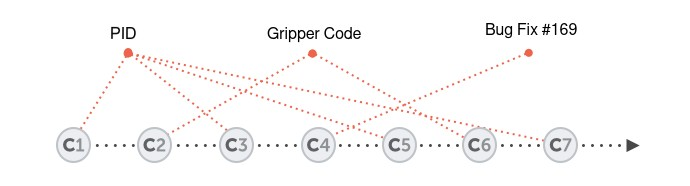
\includegraphics[width=4.5in]{images/one-context.jpg}
\end{figure}


A tempting workaround might be to simply copy your complete project folder for each new context. But this only leaves you with other problems:
\begin{itemize}
    \item You circumvent your VCS, since those new folders won't be under version control.
    \item Not being version controlled, you can't easily share \& collaborate with others.
    \item Integrating changes from one context into another (maybe your main context) is difficult and error-prone.
\end{itemize}

To make a long story short: if your goal is to maintain a level of santity, you'll have to find a way to deal with multiple contexts in a clean manner.

\subsection{Branches to the Rescue}

You might have already guessed it: branches are what we need to solve these problems. Because a branch represents exactly such a context in a project and helps you keep it separate from all other contexts.

\begin{figure}[h]
    \centering
    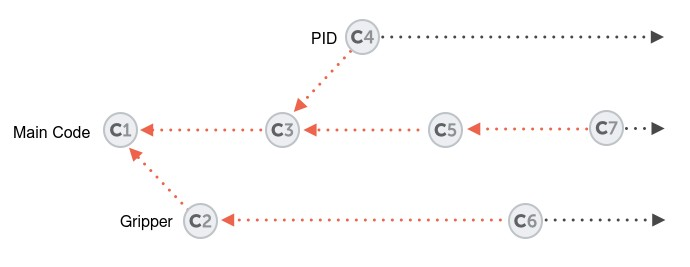
\includegraphics[width=4.5in]{images/multiple-contexts.jpg}
\end{figure}

All the changes you make at any time will only apply to the currently active branch; all other branches are left untouched. This gives you the freedom to both work on different things in parallel and, above all, to experiment - because you can't mess up! In case things go wrong you can always go back / undo / start fresh / switch contexts...
\newline\newline
Luckily, branches in Git are cheap \& easy. There's no reason not to create a new branch when you start working on a new topic, no matter how big or small it might be.

\begin{golden-rule}
Use Branches Extensively:
\newline\newline
Branching is one of Git’s most powerful features – and this is not by accident: quick and easy branching was a central requirement from day one. Branches are the perfect tool to help you avoid mixing up different lines of development. You should use branches extensively in your development workflows: for new features, bug fixes, experiments, ideas…
\end{golden-rule}

\section{Working with branches}
Until now, we haven't taken much notice of branches in our example project. However, without knowing, we were already working on a branch! This is because branches aren't optional in Git: you are always working on a certain branch (the currently active, or "checked out", or "HEAD" branch).
\newline\newline
So, which branch is HEAD at the moment? The "git status" command tells us in its first line of output: "On branch master".
The "master" branch was created by Git automatically for us when we started the project. Although you could rename or delete it, you'll have a hard time finding a project without it because most people just keep it. But please keep in mind that "master" is by no means a special or magical branch. It's like any other branch!
\newline\newline
Now, let's start working on a new feature. Based on the project's current state, we create a new branch and name it "pid-test":
\begin{lstlisting}
$ git branch pid-test
\end{lstlisting}
Using the "git branch" command lists all of our branches (and the "-v" flag provides us with a little more data than usual):
\begin{lstlisting}
$ git branch -v
  pid-test     3de33cc Got the robot to drive off a table consistently
* master       3de33cc [ahead 1] Got the robot to drive off a table consistently
\end{lstlisting}
You can see that our new branch "pid-testm" was created and is based on the same version as "master". Additionally, the little asterisk character (*) next to "master" indicates that this is our current HEAD branch. To emphasize this: the "git branch" command only created that new branch - but it didn't make it active. Before checking out that new branch, it's a good idea to have another look at "git status" to see where we currently are:
\begin{lstlisting}
$ git status
# On branch master
# Changes not staged for commit:
#   (use "git add <file>..." to update what will be committed)
#   (use "git checkout -- <file>..." to discard changes in working 
#    directory)
#
#       modified:   dobackflip.py
#
no changes added to commit (use "git add" and/or "git commit -a")
\end{lstlisting}

Oh, right: we still have some changes in "imprint.html" in our working copy! Actually, we just wanted to start working on our new "contact-form" branch; but these changes don't belong to this feature. So what do we do with them? One way to get this work-in-progress out of the way would be to simply commit it. But committing half-done work is a bad habit.

\begin{golden-rule}Never Commit Half-Done Work
\newline\newline
You should only commit code when it’s completed. This doesn’t mean you have to complete a whole, large feature before committing. Quite the contrary: split the feature’s implementation into logical chunks and remember to commit early and often. But don’t commit just to get half-done work out of your way when you need a "clean working copy". For these cases, consider using Git’s “Stash” feature instead.
\end{golden-rule}

\section{Saving Changes Temporarily}
A commit wraps up changes and saves them permanently in the repository. However, in your day-to-day work, there are a lot of situations where you only want to save your local changes temporarily. For example, imagine you're in the middle of some changes for feature X when an important bug report comes in. Your local changes don't belong to the bugfix you're going to make. You have to get rid of them (temporarily, without losing them!) and continue working on them later.
\newline\newline
Situations like this one happen all the time: you have some local changes in your working copy that you can't commit right now - and you want or need to start working on something else. To get these changes out of your way and have a "clean" working copy, Git's "Stash" feature comes in handy

\begin{concept}
The Stash
\newline\newline 
Think of the Stash as a clipboard on steroids: it takes all the changes in your working copy and saves them for you on a new clipboard. You're left with a clean working copy, i.e. you have no more local changes.
\newline\newline 
Later, at any time, you can restore the changes from that clipboard in your working copy - and continue working where you left off.
\newline\newline 
You can create as many Stashes as you want - you're not limited to storing only one set of changes. Also, a Stash is not bound to the branch where you created it: when you restore it, the changes will be applied to your current HEAD branch, whichever this may be.
\end{concept}

Let's stash away these local changes so we have a clean working copy before starting to work on our new feature:

\begin{lstlisting}
$ git stash
Saved working directory and index state WIP on master: 
   2dfe283 Got the robot to drive off a table consistently
HEAD is now at 2dfe283 Got the robot to drive off a table consistently
\end{lstlisting}
\begin{lstlisting}
$ git status
# On branch master
nothing to commit (working directory clean)
\end{lstlisting}
The local changes in "dobackflip.py" are now safely stored on a clipboard, ready to be restored any time we want to continue working on them.
\newline\newline
You can easily get an overview of your current Stashes:
\begin{lstlisting}
$ git stash list
stash@{0}: WIP on master: 2d6e283 Implement the new login box
\end{lstlisting}

The newest Stash will always be at the top of the list, named "stash@{0}". Older Stashes have higher numbers.
\newline\newline
When you're ready to restore a saved Stash, you have two options:
\begin{itemize}
    \item Calling "git stash pop" will apply the newest Stash and clear it from your Stash clipboard.
    \item Calling "git stash apply <stashname>" will also apply the specified Stash, but it will remain saved. You can delete it later via "git stash drop <stashname>".
\end{itemize}

You can choose to not specify the Stash when using any of these commands. Then, Git will simply take the newest Stash (always "stash@{0}").

\begin{concept}
When to Stash
\newline\newline
Stashing helps you get a clean working copy. While this can be helpful in many situations, it's strongly recommended...
\newline\newline
...before checking out a different branch.
\newline
...before pulling remote changes.
\newline
...before merging or rebasing a branch.
\end{concept}

\section{Checking Out a Local Branch}
Now that we have a clean working copy, the first thing we have to do is switch to (or "check out") our newly created branch:
\begin{lstlisting}
$ git checkout pid-test
\end{lstlisting}

\begin{concept}
Checkout, HEAD, and Your Working Copy
\newline\newline
A branch automatically points to the latest commit in that context. And since a commit references a certain version of your project, Git always knows exactly which files belong to that branch.
\begin{figure}[h]
    \centering
    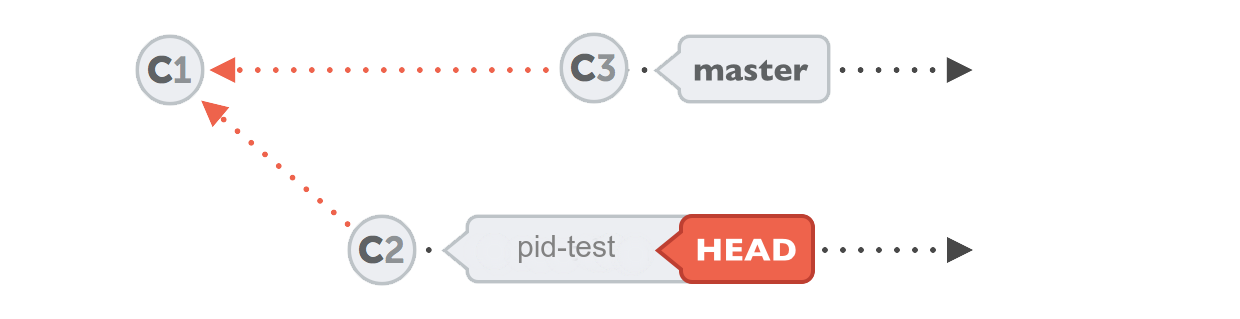
\includegraphics[width=4.5in]{images/branch-pointers.png}
\end{figure}
At each point in time, only one branch can be HEAD / checked out / active. The files in your working copy are those that are associated with this exact branch. All other branches (and their associated files) are safely stored in Git's database.
\newline\newline
To make another branch (say, "pid-test") active, the "git checkout" command is used. This does two things for you:
\begin{itemize}
    \item It makes "pid-test" the current HEAD branch.
    \item It replaces the files in your working directory to match exactly the revision that "pid-test" is at.
\end{itemize}
\end{concept}
Running "git status" once more, you'll see that we're now "On branch pid-test". From now on, all of our changes and commits will only impact this very context - until we switch it again by using the "checkout" command to make a different branch active.
\newline\newline
Let's prove this by creating a new file called "jumpboy.py" and committing it:
\begin{lstlisting}
$ git add jumpboy.py
$ git commit -m "Robot can now jump"
$ git log
commit 56eddd14cf034f4bcb8dc9cbf847b33309fa5180
Author: Arjun Gandhi <beepboop@arjungandhi.com>
Date: Fri Jul 26 10:56:16 2013 +0200

    Robot can now jump

commit 2dfe283e6c81ca48d6edc1574b1f2d4d84ae7f1
Author: Arjun Gandhi <beepboop@arjungandhi.com>
Date: Fri Jul 26 10:52:04 2013 +0200

    Got the robot to drive off a table consistently

commit 2b504bee4083a20e0ef1e037eea0bd913a4d56b6
Author: Arjun Gandhi <beepboop@arjungandhi.com>
Date: Fri Jul 26 10:05:48 2013 +0200

    Got the robot to unplug its own wires
\end{lstlisting}
Looking at the Log, you'll see that your new commit was properly saved. No big surprises, so far. But now let's switch back to "master" and have a look at the Log once more:
\begin{lstlisting}
$ git checkout master
$ git log
commit 2dfe283e6c81ca48d6edc1574b1f2d4d84ae7f1
Author: Arjun Gandhi <beepboop@arjungandhi.com>
Date: Fri Jul 26 10:52:04 2013 +0200

    Got the robot to drive off a table consistently

commit 2b504bee4083a20e0ef1e037eea0bd913a4d56b6
Author: Arjun Gandhi <beepboop@arjungandhi.com>
Date: Fri Jul 26 10:05:48 2013 +0200

    Got the robot to unplug its own wires
\end{lstlisting}

You'll find that the "Robot can now jump" commit isn't there - because we made it in the context of our HEAD branch (which was the "pid-test" branch, not the "master" branch). This is exactly what we wanted: our changes are kept in their own context, separated from other contexts.

\section{Merging Changes}
Keeping your commits in the separate context of a branch is a huge help. But there will come a time when you want to integrate changes from one branch into another. For example when you finished developing a feature and want to integrate it into your "production" branch. Or maybe the other way around: you're not yet finished working on your feature, but so many things have happened in the rest of the project in the meantime that you want to integrate these back into your feature branch.
\newline\newline
Whatever the scenario may be: such an integration is called "merging" and is done with the "git merge" command.
\begin{concept}
Integrating Branches - Not Individual Commits
\newline\newline
When starting a merge, you don't have to (and cannot) pick individual commits that shall be integrated. Instead, you tell Git which branch you want to integrate - and Git will figure out which commits you don't have in your current working branch. Only these commits will then be integrated as a result.
\newline\newline
Also, you never have to think long and hard about where these changes end up: The target of such an integration is always your current HEAD branch and, thereby, your working copy.
\begin{figure}[h]
    \centering
    \includegraphics{}
\end{figure}
\end{concept}


\begin{thebibliography}{9}
\bibitem{git-tower}
A large portion of this document was "liberated" from:
https://www.git-tower.com/learn/git/ebook/en/command-line/basics/why-use-version-control
\bibitem{atlassian}
https://www.atlassian.com/git/tutorials/what-is-git
\end{thebibliography}



\end{document}
